\documentclass[11pt]{report}

\usepackage{mathptmx}
\usepackage{url}
\usepackage{graphicx}

\newcommand*{\p}[1]{\textup{\texttt{#1}}}
\newcommand*{\ls}{\textsc{LearnSAT}}
\newcommand*{\pl}{\textsc{Prolog}}
\newcommand*{\sw}{\textsc{SWI-Prolog}}
\newcommand*{\dt}{\textsc{dot}}

\textwidth=15cm
\textheight=22cm
\topmargin=0pt
\headheight=0pt
\oddsidemargin=1cm
\headsep=0pt
\renewcommand{\baselinestretch}{1.1}
\setlength{\parskip}{0.20\baselineskip plus 1pt minus 1pt}
\parindent=0pt

\author{\bfseries Mordechai (Moti) Ben-Ari\\\url{http: //www.weizmann.ac.il/sci-tea/benari/}}
\title{\bfseries \ls\\\mbox{}\\
\bfseries\large User's Guide\\\mbox{}\\
\bfseries\normalsize Version 1.2.0}

%\date{}
\begin{document}

\maketitle

\thispagestyle{empty}

\vspace*{\fill}

\begin{center}
Copyright \copyright{} 2012 by Mordechai (Moti) Ben-Ari.
\end{center}
This work is licensed under the Creative Commons Attribution-ShareAlike 3.0
License. To view a copy of this license, visit
\url{http://creativecommons.org/licenses/by-sa/3.0/}; or, (b) send a letter
to Creative Commons, 543 Howard Street, 5th Floor, San Francisco,
California, 94105, USA.

\bigskip

 
\begin{center}
The following copyright notice applies to the programs described in this
document:\mbox{}\\\mbox{}\\
Copyright 2012 by Mordechai (Moti) Ben-Ari.
\end{center}

This program is free software; you can redistribute it and/or
modify it under the terms of the GNU General Public License
as published by the Free Software Foundation; either version 2
of the License, or (at your option) any later version.
This program is distributed in the hope that it will be useful
but WITHOUT ANY WARRANTY; without even the implied warranty of
MERCHANTABILITY or FITNESS FOR A PARTICULAR PURPOSE.
See the GNU General Public License for more details.
You should have received a copy of the GNU General Public License
along with this program; if not, write to the Free Software
Foundation, Inc., 59 Temple Place - Suite 330, Boston, MA
02111-1307, USA.

\vspace*{\fill}

\tableofcontents

\thispagestyle{empty}

\setcounter{page}{0}


\newpage

\section*{Overview}\addcontentsline{toc}{section}{\textbf{Overview}}

\ls{} is a program for learning about SAT solving. It implements the
classic \emph{Davis-Putnam-Logemann-Loveland (DPLL)} algorithm, together
will modern extensions of the algorithm: \emph{conflict-driven clause
learning (CDCL)} and \emph{non-chronological backtracking (NCB)}.

For a gentle introduction to SAT solvers, see \cite[Chapter~6]{mlcs}.
The comprehensive reference is the \emph{Handbook of Satisfiability}
\cite{SAT}. The algorithms and notation of \ls{} follow \cite{mlm}.

The design of \ls{} is based on the following principles:

\begin{itemize}

\item A very detailed trace of the algorithm's execution can be
displayed. The content of the trace can be set by the user.

\item The \pl{} language is used so that the programs will be concise
and easy to understand, but only a little knowledge of \pl{} is needed
just to run the program.

\item A utility is provided for converting between sets of clauses
represented as \pl{} terms and those in DIMACS format. While the former
are easier to read, existing examples in DIMACS format can be downloaded
and converted.

\item \ls{} is an open-source project.
\end{itemize}

The three chapters of this document are a user's guide, a short tutorial
on SAT solving with \ls{} and documentation of the software.


\chapter{User's Guide}

\section{Installation}

\ls{} can be downloaded from Google Code at:\footnote{This project also
contains an archive of \pl{} programs for the algorithms in my textbook
\emph{Mathematical Logic for Computer Science (Third Edition)}
\cite{mlcs}.}
\begin{center}
\url{http://code.google.com/p/mlcs/}.
\end{center}

Download and open the zip archive \p{learnsat-N.zip}. The \pl{} source
code in the directory \p{src} and the documentation is in the directory
\p{docs}.

Download and install \sw{}:\footnote{The program was developed using
Version 6.0.0.}
\begin{center}
\url{http://www.swi-prolog.org/}.
\end{center}

The source files use the extension \p{pro} instead of the more usual
\p{pl} to avoid conflict with programs in Perl. During the installation
of \sw{}, if you associate the extension \p{pro} with \sw{}, a
program can be launched by double-clicking on its name in a file list. 

The main module is file \p{dpll.pro}. It exports the predicates shown in
Table~\ref{tab.export}.

\begin{table}
\begin{center}
\begin{tabular}{|l|l|}
\hline
\multicolumn{2}{|c|}{\textbf{\large Predicates}}\\
\hline
\p{dpll}&Run the DPLL algorithm\\
\p{usage}&Show the predicates, modes and display options \\
\p{show\_config}&Show the current mode and display options\\
\p{set\_display}&Set display options\\
\p{clear\_display}&Clear display options\\
\p{set\_mode}&Set the algorithmic mode\\
\p{to\_dimacs}&Convert from \pl{} term to DIMACS\\
\p{from\_dimacs}&Convert from DIMACS to \pl{} term\\
\hline
\end{tabular}
\end{center}
\caption{Exported predicates}\label{tab.export}
\end{table}


\section{Running \ls}

\subsection{Creating a file to check satisfiability}

To check the satisfiability of a CNF formula, create a \pl{} program
that calls the predicate \p{dpll} with the set of clauses represented as
a list of lists of literals.

The file with the program must be in the \p{src} directory or the \ls{}
source files must be copied to the directory that contains that file.

Here is a program for the pigeon-hole problem for two holes and three
pigeons, where \p{pij} means that pigeon \p{i} is in hole \p{j}:

\begin{verbatim}
:- use_module(dpll).

hole2 :-
  dpll(
  [
  [p11, p12],   [p21, p22],   [p31, p32],   % Each pigeon in hole 1 or 2 
  [~p11, ~p21], [~p11, ~p31], [~p21, ~p31], % No pair is in hole 1
  [~p12, ~p22], [~p12, ~p32], [~p22, ~p32], % No pair is in hole 2
  ], _).
\end{verbatim}

The result (a satisfying assignment or \p{[]} if unsatisfiable) is
returned as the second argument, but can be left anonymous if only
the trace is of interest.

\subsection{Loading and running a file}

Once this file has been loaded (by double-clicking or by consulting
\p{[pigeon]}), the query \p{hole2} can be run. After the execution
terminates with \p{true} you must press return to get a new prompt. The
output will be a trace of the DPLL algorithm (Figure~\ref{fig.pigeon}).

The user cannot control the order of decision assignments; lexicographic
order of the variable names is used.

\begin{figure}[tbp]
\begin{verbatim}
?- hole2.
LearnSAT v1.1.0. Copyright 2012 by Moti Ben-Ari. GNU GPL.
Decision assignment: p11=0
Propagate unit p12 derived from: 1. [p11,p12]
Propagate unit ~p22 derived from: 7. [~p12,~p22]
Propagate unit p21 derived from: 2. [p21,p22]
Propagate unit ~p31 derived from: 6. [~p21,~p31]
Propagate unit p32 derived from: 3. [p31,p32]
Conflict clause: 8. [~p12,~p32]
Decision assignment: p11=1
                ...
Unsatisfiable
Clauses=9, variables=6, units=56, decisions=12, conflicts=12

true.
\end{verbatim}
\caption{Running the program for the pigeon-hole principle}\label{fig.pigeon}
\end{figure}

The trace output can be directed to a file:

\begin{verbatim}
hole2_file :- tell('hole2.txt'), hole2, told.
\end{verbatim}

\subsection{Algorithmic modes}

\ls{} can run in one of three modes set by the predicate \p{set\_mode(Mode)}
(Table~\ref{tab.modes}).

The default mode can be changed by editing the file \p{config.pro}.

The pigeon-hole program runs much more efficiently in \p{cdcl} mode:
\begin{verbatim}
?- set_mode(cdcl).
true.
?- hole2.
                ...
Unsatisfiable:
Statistics: clauses=9, variables=6, units=29, decisions=12, conflicts=12
\end{verbatim}

\begin{table}[*b]
\begin{center}
\begin{tabular}{|l|l|}
\hline
\multicolumn{2}{|c|}{\textbf{\large Modes}}\\
\hline
\p{dpll} & DPLL algorithm (default)\\
\p{cdcl} & DPLL with conflict-directed clause learning\\
\p{ncb} &  DPLL with CDCL and non-chronological backtracking\\
\hline
\end{tabular}
\caption{\ls{} modes}\label{tab.modes}
\end{center}
\end{table}

\subsection{Display options}

\ls{} writes extensive trace output as it executes the algorithms. Each
line starts with a string followed by a colon to make it easy to
postprocess the output. The content of the trace is controlled using
\p{set\_display} and \p{clear\_display}. The argument to these
predicates can be \p{all} or \p{default} or a single option or a list of
options taken from Table~\ref{tab.display}. The default options can be
changed by editing the file \p{config.pro}.

If you need to change the mode and options frequently, you
can write a predicate to do so:
\begin{verbatim}
ncb_mode :- set_mode(ncb), set_display([antecedent, graph, skipping, uip]).
\end{verbatim}


In \p{cdcl} and \p{ncb} modes, the assignments are written together with
their levels in the format \p{p1=0@3} used in \cite{mlm}. Optionally,
the antecedent clause can be displayed with each assignment:
\verb+p1@3/[~p1,p3]+.

\begin{table}
\begin{center}
\begin{tabular}{|l|l|}
\hline
\multicolumn{2}{|c|}{\textbf{\large Display options}}\\
\hline
\p{all}       &  all of the options\\
\p{default}   &  default options (indicated by *)\\
\hline
\p{antecedents}&  antecedents of each assigned atom\\
\p{assignments}& assignments that caused a conflict         \\
\p{backtrack}*&  level of non-chronological backtracking    \\
\p{clauses}   &  clauses to be checked for satisfiability   \\
\p{conflict}* &  conflict clauses                           \\
\p{decision}* &  decision assignments                       \\
\p{dominator} &  learned clause computed from dominator     \\
\p{evaluate}  &  evaluation of clauses for an assignment    \\
\p{dot}       &  implication graphs in dot format           \\
\p{graph}     &  implication graphs                         \\
\p{incremental}& incremental build of the implication graphs\\
\p{learned}*  &  learned clauses                            \\
\p{literal}   &  literals found assigned during CDCL        \\
\p{partial}   &  partial assignment so far                  \\
\p{resolvent} &  resolvents created during CDCL             \\
\p{result}*   &  result of the algorithm                    \\
\p{skipping}  &  assignments skipped when backtracking      \\
\p{uip}       &  unique implication points                  \\
\p{unit}*     &  unit clauses                               \\
\p{variables} &  variables that are not assigned so far     \\
\hline
\end{tabular}
\end{center}
\caption{Display options}\label{tab.display}
\end{table}

\subsection{Online help}

The predicate \p{usage} shows the commands, and the mode and display
arguments.

The version, the default and current mode, and the default and current
display options can be shown by running \p{show\_config}.

\subsection{Rendering the implication graphs}\label{s.impl}

\ls{} constructs the implication graph when a conflict clause is
encountered and the graph can be displayed (both the final graph and the
graphs that are incrementally constructed). 
The graph can
also be written to a file in \dt{} format which can be rendered using
\textsc{GraphViz}:\footnote{\url{http://www.graphviz.org/}.}

\begin{verbatim}
dot -Tpng examples-00.dot > examples-00.png
\end{verbatim}
You can choose to label the edges with clause numbers as in \cite{mlm}
or with the clauses themselves.

A script to run \dt{} on all the files for the incremental graphs; for
example, in Windows:
\begin{verbatim}
for %%F in (*.dot) do c:\...\graphviz\bin\dot -Tpng %%F > %%~nF.png
\end{verbatim}

The \dt{} prologue and the decoration of decision nodes can be set in
\p{config.pro}.


\section{Test programs included in \ls{}}

\begin{itemize}
\item \p{examples.pro} contains examples from papers on SAT
solvers \cite{mz,mlm,ms}.

\item \p{tseitin.pro}: Tseitin clauses for $K_{2,2}$,
$K_{3,3}$ and the example from \cite[Section 4.5]{mlcs}.

\item \p{queens.pro}: The four-queens problem.

\item \p{pigeon.pro}: The pigeon-hole principle for two and three holes.

\item \p{pebbles.pro}: Grid pebbling for depth 2 and 3.
\end{itemize}


\section{DIMACS transformation}

The predicates in the file \p{dimacs.pro} convert a set of clauses in
\pl{} format (a list of lists of literals) to and from \emph{simplified
DIMACS cnf format} that is used by SAT solvers.
\begin{itemize}
\item \p{to\_dimacs(File, Comment, Clauses)} converts the \pl{}
\p{Clauses} into DIMACS format and writes them to the \p{File} with the
\p{Comment}.
\item \p{from\_dimacs(Predicate, InFile, OutFile)} reads \p{InFile} in
DIMACS format and converts the data into a program written on
\p{OutFile}. \p{Predicate} is the name to be given to the predicate for
running \p{dpll}:
\begin{verbatim}
Predicate :- dpll(List, _).
\end{verbatim}
\end{itemize}




\chapter{Tutorial}

For the tutorial, we will used the set of clauses from \cite{mlm} as our
example:\footnote{The file \p{examples.pro} contains the predicate
\p{mlm} that runs \p{dpll} on this set of clauses.}

\begin{verbatim}
  1. [x1,x031,~x2]   2. [x1,~x3]         3. [x2,x3,x4]
  4. [~x4,~x5]       5. [x021,~x4,~x6]   6. [x5,x6]
\end{verbatim}

Since \ls{} tries decision assignments in lexicographic order, two
clauses have a \p{0} added to ensure that they are chosen first.

\section{The DPLL algorithm}

When the DPLL algorithm is applied to the set of clauses, it assigns
0 to \p{x021}, \p{x031} and \p{x1}:

\begin{verbatim}
?- mlm.
LearnSAT v1.2.0. Copyright 2012 by Moti Ben-Ari. GNU GPL.
Decision assignment: x021=0
Decision assignment: x031=0
Decision assignment: x1=0
\end{verbatim}

Clause 1 is now a unit clause implying that \p{x2} must be assigned 0.
This in turn leads to a sequence of unit propagations until clause 6 is
falsified:
\begin{verbatim}
Propagate unit: ~x2 derived from: 1. [x1,x031,~x2]
Propagate unit: ~x3 derived from: 2. [x1,~x3]
Propagate unit: x4 derived from: 3. [x2,x3,x4]
Propagate unit: ~x5 derived from: 4. [~x4,~x5]
Propagate unit: ~x6 derived from: 5. [x021,~x4,~x6]
Conflict clause: 6. [x5,x6]
\end{verbatim}

The algorithm backtracks, trying the assignment of 1 to \p{x1} and then
0 to \p{x2} and \p{x3}:
\begin{verbatim}
Decision assignment: x1=1
Decision assignment: x2=0
Decision assignment: x3=0
\end{verbatim}
which causes another sequence of unit propagations leading to the same
conflict clause:
\begin{verbatim}
Propagate unit: x4 derived from: 3. [x2,x3,x4]
Propagate unit: ~x5 derived from: 4. [~x4,~x5]
Propagate unit: ~x6 derived from: 5. [x021,~x4,~x6]
Conflict clause: 6. [x5,x6]
\end{verbatim}

The algorithms backtracks to assign 1 to \p{x3}, followed by 0 to \p{x4}
and \p{x5}, and the propagation of a unit; the result is a set of
assignments that satisfies the set of clauses:
\begin{verbatim}
Decision assignment: x3=1
Decision assignment: x4=0
Decision assignment: x5=0
Propagate unit: x6 derived from: 6. [x5,x6]
Satisfying assignments:
[x021=0,x031=0,x1=1,x2=0,x3=1,x4=0,x5=0,x6=1]
Statistics: clauses=6, variables=8, units=9, decisions=9, conflicts=2
\end{verbatim}


\section{Conflict-driven clause learning}

Let us now run the same example with CDCL after first setting
the mode and display options:\footnote{Alternatively, you
can select the display option \p{graph} instead of \p{dot} to obtain a
textual representation of the graph.}
\begin{verbatim}
?- set_mode(cdcl).
?- set_display([literal, resolvent, uip, dot]).
?- mlm.
\end{verbatim}

\subsection{The implication graph}

When the conflict clause is found the \emph{implication graph} is
generated (Figure~\ref{fig.graph}). It represents the result of unit
propagation that causes a conflict. There are three source nodes, one
for each of the decision assignments (\p{x021=0@1}, \p{x031=0@2},
\p{x1=0@3}) that are sufficient to cause a conflict by unit propagation.
The level of each decision assignment is added to the assignment in
\p{cdcl} mode.

The conflict is represented by the sink node \p{kappa} and the
assignments that were forced by unit propagation are represented by
nodes labeled with the assignments. An edge of the graph is labeled with
the number of the clause that is the \emph{antecedent} of the node; this
is the unit clause that forced the assignment labeling that
node.\footnote{The display option \p{antecedent} will display the clause
itself in addition to its number.} There is an edge for each literal in
the unit clause (except the one whose assignment is forced) and the
sources of these edges are the assignments to those literals. For
example, the decision assignments \p{x021=0@1}, \p{x031=0@2}
cause clause 1 \verb+[x1, x031, ~x2]+ to become a unit clause
and force the assignment of 0 to \p{x2}.

\begin{figure}
\begin{center}
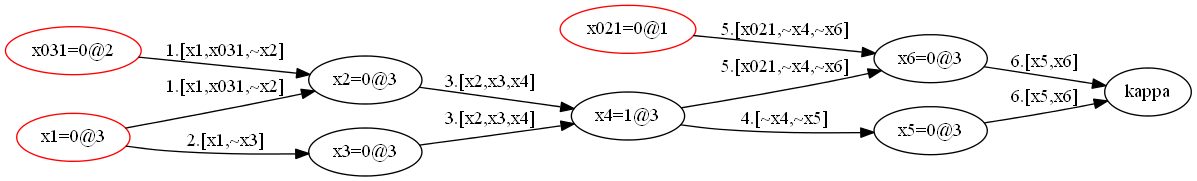
\includegraphics[keepaspectratio=true,width=\textwidth]{graph}
\end{center}
\caption{Implication graph}\label{fig.graph}
\end{figure}

\subsection{Learning a clause from dominators}

Learning the clause \p{[x021, x031, x1]} defined by the complements of
the decision assignments will ensure that this computation is never
tried again. However, a better clause to learn is defined by a
\emph{unique implication point (UIP)}. Consider all the paths from the
last decision assignment \p{x1=0@3} to the kappa node. All these paths
pass through the dominator (the node \p{x4=1@3}), which is called a UIP.
This assignment is implied by \p{x031=0@2} and \p{x1=0@3}. Therefore,
learning the clause \p{[x021,~x4]} will also prevent the computation
defined by these decisions. To display the generation of the learned
clause, select the display option \p{dominator}:

\begin{verbatim}
Paths from the decision node at this level to kappa:
x1=0@3 --> x2=0@3 --> x4=1@3 --> x5=0@3 --> kappa
x1=0@3 --> x2=0@3 --> x4=1@3 --> x6=0@3 --> kappa
x1=0@3 --> x3=0@3 --> x4=1@3 --> x5=0@3 --> kappa
x1=0@3 --> x3=0@3 --> x4=1@3 --> x6=0@3 --> kappa
A dominator is: x4=1@3
Decisions at a lower level: [assign(x021,0,1,yes),assign(x031,0,2,yes)]
Decisions not dominated: [assign(x021,0,1,yes)]
\end{verbatim}

This method of learning a clause is performed only for display purposes;
the learned clause that is used is determined by a different method
described in the next subsection.

\subsection{Learning a clause by resolution}

The conflict clause (the antecedent clause of the \p{kappa} node) is defined
as the current clause and resolution is carried out until a UIP is found.
The clause to be resolved with the current clause is one that clashes on a literal
that is assigned at the current level \emph{by unit propagation}. For
example, given the conflict clause \p{[x5,x6]}, both
\p{x5} and \p{x6} were assigned by unit propagation at this level, so we
can successively resolve \p{[x5,x6]} with the antecedent clauses of the
assignments, namely, \verb+[~x4,~x5]+ and then \verb+[x021,~x4,~x6]+ (or
in the opposite order). 

The resolution terminates when a \emph{unique
implication point (UIP)} is encountered; this is a clause where only one
literal is assigned at the current level. This clause is the
\emph{learned clause} and is added to the list that is the argument of
the single fact in the database \p{learned}. In the example, the learned
clause is \verb+[x021,~x4]+.

The second clause for each resolution step is one that clashes with the
current clause on a literal that is assigned at the current level
\emph{by unit propagation}. For example, given the conflict clause
\p{[x5,x6]}, \p{x5} was assigned by unit propagation at this level, so
we can resolve \p{[x5,x6]} with the antecedent clause of the assignments
\verb+[~x4,~x5]+ to obtain the resolvent \verb+[x6,~x4]+ which is also a
conflict clause. The next step is to resolve with \verb+[x021,~x4,~x6]+
to obtain \verb+[x021,~x4]+.\footnote{The resolutions could also be done
in the opposite order with the same result.} The resolution now
terminates because clause is a UIP, namely, a clause where only one
literal is assigned at the current level. The \ls{} output is:

\begin{verbatim}
Literal: x5 assigned at level: 3
Literal: x6 assigned at level: 3
Not a UIP: two literals are assigned at level: 3
Clause: [x5,x6] unsatisfied
Complement of: x5 assigned true in the unit clause: [~x4,~x5]
Resolvent of the two clauses: [x6,~x4] is also unsatisfiable
Literal: x6 assigned at level: 3
Literal: ~x4 assigned at level: 3
Not a UIP: two literals are assigned at level: 3
Clause: [x6,~x4] unsatisfied
Complement of: x6 assigned true in the unit clause: [x021,~x4,~x6]
Resolvent of the two clauses: [x021,~x4] is also unsatisfiable
Literal: ~x4 assigned at level: 3
UIP: one literal is assigned at level: 3
Learned clause: [x021,~x4]
\end{verbatim}

The DPLL algorithm now continues as before but with the learned clause
added to the set of clauses. The result is that a satisfying assignment
is found more efficiently with fewer decisions (6 instead of 9):

\begin{verbatim}
Decision assignment: x1=1@3
Propagate unit: ~x4 derived from: 7. [x021,~x4]
Decision assignment: x2=0@4
Propagate unit: x3 derived from: 3. [x2,x3,x4]
Decision assignment: x5=0@5
Propagate unit: x6 derived from: 6. [x5,x6]
Satisfying assignments:
[x021=0@1/nil,x031=0@2/nil,x1=1@3/nil,x2=0@4/nil,
 x3=1@4/[x2,x3,x4],x4=0@3/[x021,~x4],x5=0@5/nil,x6=1@5/[x5,x6]]
Statistics: clauses=6, variables=8, units=8, decisions=6, conflicts=1
\end{verbatim}


\section{Non-chronological backtracking}

Let us now select the NCB mode and the display of the skipped variables:
\begin{verbatim}
?- set_mode(ncb).
?- set_display(skipping).
?- mlm.
\end{verbatim}

When a learned clause has been obtained, the backtrack level for
non-chronological backtracking is computed. This is the highest level of
an assignment in the learned clause except for the current level.
The DPLL algorithm skips decision assignments whose level is at a lower
level than the backtrack level. In the example, the highest level is 1
where \p{x021} was assigned:

\begin{verbatim}
Non-chronological backtracking to level: 1
Skip decision assignment: x1=1@3
Skip decision assignment: x031=1@2
\end{verbatim}

For this example, there is no difference between CDCL with and without
NCB, but for the three-hole pigeon-hole principle, this difference is
significant:
\begin{verbatim}
Statistics: clauses=22, variables=12, units=243, decisions=96, conflicts=91

Statistics: clauses=22, variables=12, units=105, decisions=34, conflicts=26
\end{verbatim}




\chapter{Software documentation}

\section{Module structure}

The \ls{} software consists of the following source files:\footnote{The
list does not including the test programs and the program for DIMACS
conversion discussed above.}

\begin{itemize}
\item \p{dpll.pro}: Main module for the DPLL algorithms.
The negation operator is defined as \verb+op(610, fy, ~)+ and exported.

\item \p{auxpred.pro}: Auxiliary predicates for the DPLL algorithms. 

\item \p{io.pro}: Predicates for writing: (a) assignments; (b) clauses;
(c) implication graphs.

\item \p{display.pro}: Display the trace using predicates \p{display/n},
where the first argument is a display option and the additional
arguments supply the data to be displayed.

\item \p{config.pro}: Default configuration data. The module contains
the facts: \p{version}, \p{years}, \p{default\_mode},
\p{default\_display}, \p{dot\_prologue}, \p{dot\_decorate}.

\item \p{counters.pro}: Maintains and displays counters for units,
decisions and conflicts, as well as a counter for adding a number to the
file names for implication graphs.

\item \p{modes.pro}: Sets, clears and checks the execution mode and the
display options. It also implements \p{usage} and \p{show\_config}. The
dummy display option \p{none} is used to distinguish between the initial
state (no options, so set the default options) and a state where all
options have been cleared.

\end{itemize}

\newpage

\section{The DPLL algorithm}

The predicate \p{dpll/2} implements the DPLL algorithm on a set of clauses
represented as a list of lists of literals. It always succeeds,
returning either a list of satisfying assignments or the empty list if
the clauses are unsatisfiable. As part of its initialization, the set of
variables in the clauses is obtained from the list. 

The predicate \p{dpll/2} invokes \p{dpll/6} which is the main recursive
predicate for performing the algorithm. If the set of variables is
empty, the set of clauses is unsatisfiable. Otherwise, \p{dpll/6} tries
to perform unit propagation by searching for a unit and then evaluating
the set of clauses. When no more units remain, it chooses a decision
assignment and evaluates the set of clauses.

The predicate \p{ok\_or\_conflict} is called with the result of the
evaluation of unit propagation or the choice of an assignment. If the
result is not a conflict clause, the variable chosen is deleted and
\p{dpll/6} is called recursively. If there was a conflict clause, the
implication graph is constructed and a learned clause is generated from
the graph; then \p{ok\_or\_conflict} fails so that backtracking can try
a new assignment.

\p{evaluate} a set of clauses; returns \p{ok} or \p{conflict}.

\p{evaluate\_clause} returns one of \p{satisfied}, \p{unsatisfied},
\p{unit}, \p{unresolved}.

\p{choose\_assignment} returns an assignment and backtracking is used to
return subsequent choices. The predicate \emph{Condition} $\rightarrow$
\emph{Action} with an internal \p{!, fail} implements non-chronological
backtracing. (See the comments and Section~4.7 of the \sw{} Reference
Manual.)


\section{CDCL and NCB}

The implication graph is built incrementally. Whenever a unit clause is
found, the predicate \p{extend\_graph} is called with the unit clause,
its number (to label the new edges), the assignment it forces (to create
the new target of the edges) and the graph constructed so far. For each
literal (except the one implied), a new edge is created and when the
list of literals has been traversed, the new node is created. When a
conflict is encountered, the \p{kappa} node and its incoming edges are
added and the graph is passed to \p{compute\_learned\_clause\_by\_resolution}.

The predicate \p{compute\_learned\_clause\_by\_resolution} starts with
the conflict clause (the antecedent clause of the \p{kappa} node) as the
current clause. In \p{compute\_learned\_clause}, a search is made for a
clause that contains the complement of a literal in the current clause
and which is assigned at the current level using unit propagation, that
is, it is not a decision node. \p{resolve} computes the resolven of the
two clauses and \p{compute\_learned\_clause} is called with the
resolvent as the new current clause.

The resolution terminates when \p{check\_uip} identifies the current
clauses as a UIP. This clause is the learned clause and the predicate
\p{compute\_learned\_clause\_by\_resolution} adds it to the list that is
the argument of the fact \p{learned}.

\p{compute\_learned\_clause\_by\_dominator} displays the computation of
a learned clause by locating a dominator of the highest-level decision
assignment node relative to the \p{kappa} node.\footnote{The computation
is performed only for display (display option \p{dominator}); the
learned clause computed by resolution is the one that is used.}
\p{findall} with \p{get\_path} returns a list of all paths from the
decision node to the \p{kappa} node. This list is an argument to
\p{get\_dominator} which finds a node that appears on all the paths.
\p{findall} with \p{lower\_decision\_assignment} creates a list of all
decision nodes at lower levels and then \p{findall} is called with
\p{no\_path} to extract those nodes with no path to the dominator. The
learned clause is the complement of that assignment together with the
complements of all decision assignments not dominated by the dominator.

When a learned clause has been obtained, \p{compute\_backtrack\_level}
returns the highest level of an assignment in the learned clause except
for the current level. The level is stored as the fact \p{backtrack}.


\section{Auxiliary predicates}\label{s.aux}

\begin{itemize}

\item \p{is\_assigned} checks if a literal is assigned a value
and if so returns that value (0 or 1).

\item \p{literals\_to\_variables} takes a list of literals and returns a
sorted set of the variables corresponding to the literals.

\item \p{to\_variable} returns the variable of a literal and
\p{to\_complement} returns the complement of a literal.

\item \p{to\_assignment} and \p{to\_literal} convert to and from a
literal and an assignment expressed as a term \p{assign(Variable, Value,
Level, Decision)}, where \p{Level} is the level at which the assignment
was made and \p{Decision} is \p{yes} if the assignment was
made as a decision and \p{no} if the assignment was the result of unit
propagation.

\item \p{to\_clause} converts a list of assignments to a clause---a list
of literals. It can optionally complement each literal.

\end{itemize}


\bibliographystyle{plain}
\bibliography{learnsat}
\end{document}
